\textbf{خرد جمعی}

می‌دانیم که Adaboost یک دسته‌بند \(H\) را با استفاده از جمع وزن‌دار یادگیرنده‌های ضعیف \(h_t\) به صورت زیر یاد می‌گیرد:

\begin{latin}
    
\[
H(x) = \operatorname{sgn} \left( \sum_{t=1}^T \alpha_t h_t(x) \right)
\]
\end{latin}


در این سوال، ما از درخت‌های تصمیم به عنوان یادگیرنده‌های ضعیف خود استفاده می‌کنیم، که یک نقطه را به عنوان \(\{1, -1\}\) بر اساس دنباله‌ای از \lr{threshold}ها روی ویژگی‌های آن (اینجا \(x, y\)) طبقه‌بندی می‌کنند.

در سوالات زیر فرض کنید 
 که در صورت برابری امتیاز برای کلاس مثبت و منفی، خروجی دسته‌بندها به طور دلخواه تعیین می‌شود.
\vspace{-5mm}
\begin{enumerate}
\item
فرض کنید یادگیرنده‌های ضعیف ما درخت‌های تصمیم با عمق 1 هستند (\lr{Decision Stumps})، که خطای آموزشی وزن‌دار را کمینه می‌کنند. با استفاده از مجموعه داده زیر، مرز تصمیمی که توسط \(h_1\) یاد گرفته شده است را ترسیم کنید.
\vspace{-5mm}
\begin{figure}[H]
    \latin
    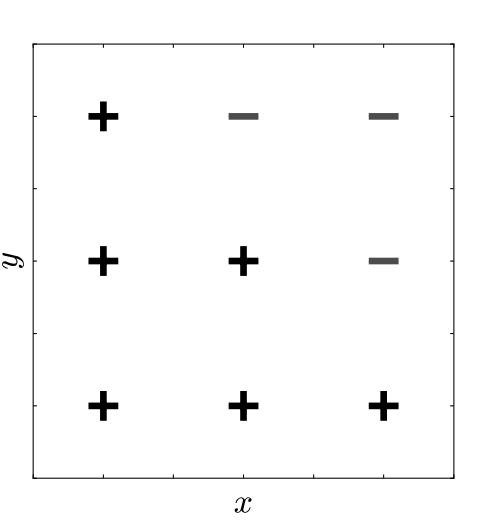
\includegraphics[width=0.28\linewidth,left]{images/2-1.png}
\end{figure}
\vspace{-5mm}
\item
 در مجموعه داده‌ی زیر، نقطه(های) با بیشترین وزن در \lr{iteration} دوم را مشخص و مرز تصمیمی که توسط \(h_2\) یاد گرفته شده است را ترسیم کنید.
 \vspace{-5mm}
\begin{figure}[H]
    \latin
    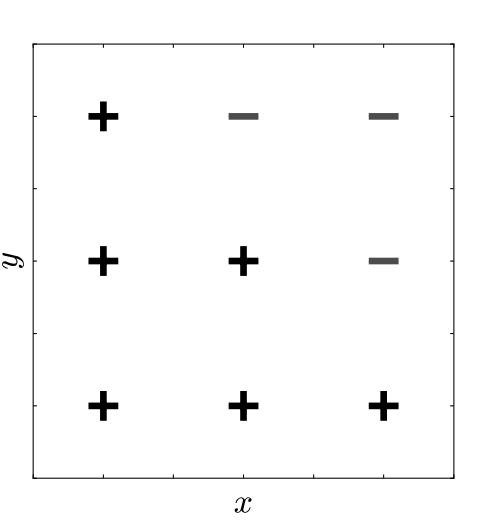
\includegraphics[width=0.28\linewidth,left]{images/2-1.png}
\end{figure}
\vspace{-5mm}
\item
در مجموعه داده‌ی زیر، مرز تصمیم \(H = \operatorname{sgn} (\alpha_1 h_1 + \alpha_2 h_2)\) را ترسیم کنید. (راهنمایی: نیازی به محاسبه صریح \(\alpha\) ها نیست).
\vspace{-5mm}
\begin{figure}[H]
    \latin
    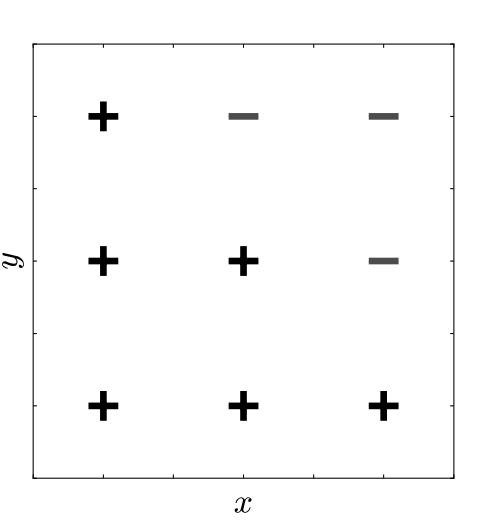
\includegraphics[width=0.28\linewidth,left]{images/2-1.png}
\end{figure}
\vspace{-5mm}
\item
اکنون فرض کنید که یادگیرنده‌های ضعیف ما درخت‌های تصمیم با عمق حداکثر 2 هستند، که خطای آموزشی وزن‌دار را کمینه می‌کنند. با استفاده از مجموعه داده‌ی زیر، مرز تصمیمی که توسط \(h_1\) یاد گرفته شده است را ترسیم کنید.
\begin{figure}[H]
    \latin
    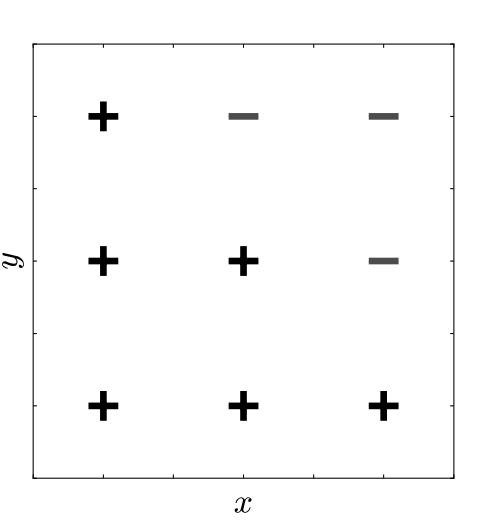
\includegraphics[width=0.28\linewidth,left]{images/2-1.png}
\end{figure}
\vspace{-5mm}
\item
 در مجموعه داده‌ی زیر، نقطه(ها) با بیشترین وزن در \lr{iteration} دوم را دایره بکشید و مرز تصمیمی که توسط \(h_2\) یاد گرفته شده است را ترسیم کنید.
\vspace{-5mm}
\begin{figure}[H]
    \latin
    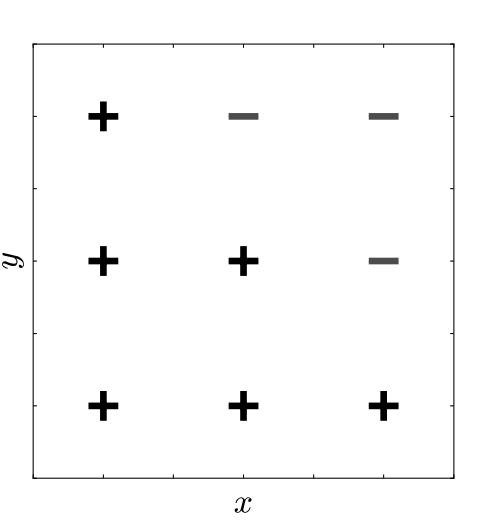
\includegraphics[width=0.28\linewidth,left]{images/2-1.png}
\end{figure}
\vspace{-5mm}
\item
در مجموعه داده‌ی زیر، مرز تصمیم \(H = \operatorname{sgn} (\alpha_1 h_1 + \alpha_2 h_2)\) را ترسیم کنید. (راهنمایی: نیازی به محاسبه صریح \(\alpha\) ها نیست).
\vspace{-5mm}
\begin{figure}[H]
    \latin
    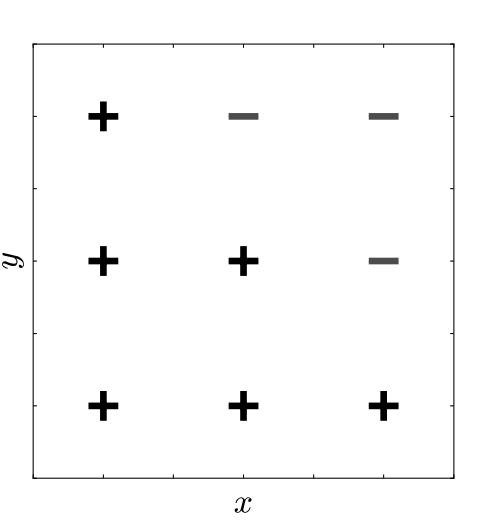
\includegraphics[width=0.28\linewidth,left]{images/2-1.png}
\end{figure}
\end{enumerate}